\documentclass{article}%
\usepackage[T1]{fontenc}%
\usepackage[utf8]{inputenc}%
\usepackage{lmodern}%
\usepackage{textcomp}%
\usepackage{lastpage}%
\usepackage[head=40pt,margin=0.5in,bottom=0.6in]{geometry}%
\usepackage{graphicx}%
%
\title{\textbf{Médicos exigen que se respete el contrato colectivo}}%
\author{El Nacional}%
\date{17/10/2018}%
%
\begin{document}%
\normalsize%
\maketitle%
\textbf{URL: }%
http://www.el{-}nacional.com/noticias/salud/medicos{-}exigen{-}que{-}respete{-}contrato{-}colectivo\_256074\newline%
%
\textbf{Periodico: }%
EN, %
ID: %
256074, %
Seccion: %
Salud\newline%
%
\textbf{Palabras Claves: }%
Salud\newline%
%
\textbf{Derecho: }%
2.1%
, Otros Derechos: %
2.3%
, Sub Derechos: %
2.1.1, 2.3.4%
\newline%
%
\textbf{EP: }%
SI\newline%
\newline%
%
\textbf{\textit{El salario no es suficiente para alimentar a una familia ni para cubrir el transporte público, dijo el médico Carlos Prosperi, en la protesta en el J M de los Ríos}}%
\newline%
\newline%
%
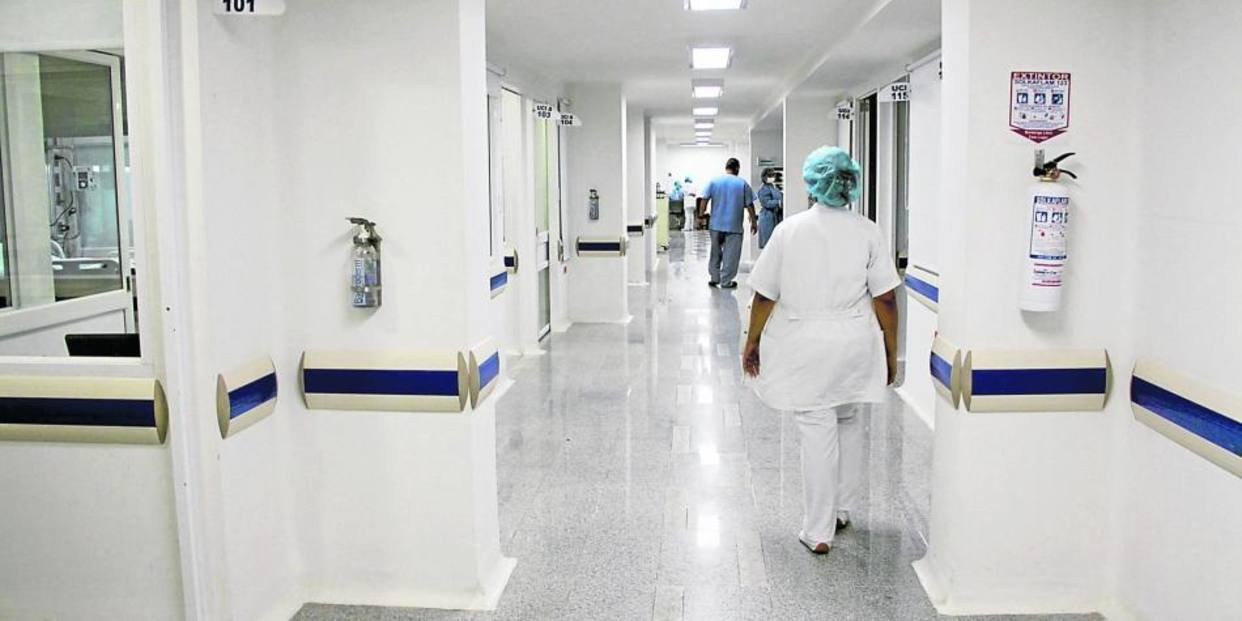
\includegraphics[width=300px]{19.jpg}%
\newline%
%
Gremios de la salud protestaron ayer en el Hospital J. M. de los Ríos para exigir el respeto al contrato colectivo que establece la tabla salarial.%
\newline%
%
Carlos Prosperi, presidente de~la Sociedad~de Médicos Internos y Residentes del Hospital Vargas, indicó que el salario de un profesional no es suficiente para pagar la alimentación ni cubrir los pasajes del transporte público. “Los que nos trasladamos desde lejana procedencia tenemos que pagar hasta cinco autobuses para llegar a nuestro destino y hoy en día no contamos con los recursos suficientes ni con un sueldo justo~para transportarnos al trabajo ni alimentar a nuestras familias”, destacó.%
\newline%
%
Denunció que el gobierno es el responsable de la crisis en salud por no dar respuestas sobre los insumos que se necesitan en los hospitales.%
\newline%
%
Las fallas eléctricas que se presentaron en el país el lunes pasado también afectaron la región capital, y los pacientes del centro pediátrico padecieron sus severas consecuencias. “Los niños que estaban en la unidad de cuidados intensivos en el J. M. de los Ríos sufrieron la indolencia y la incapacidad de un gobierno que ha dejado de meter la mano a los hospitales, porque no los dotan de insumos, ni mucho menos han mejorado los equipos médicos”, manifestó Prosperi.%
\newline%
%
Alegó que ese día las enfermeras y camareros tuvieron que hacer lo posible para que la planta eléctrica funcionara y controlar la situación con los pequeños. “Esos pacienticos pudieron perder la vida, unos niños que apenas están empezando a vivir y son los más vulnerables, por culpa de un gobierno incapaz”, expresó.%
\newline%
%
Bioanalistas~en crisis.~Ayer los gremios en~la Maternidad Concepción~Palacios, en Caracas, también alzaron su voz en las calles para exigir mejoras salariales y el cumplimiento del contrato colectivo.~“El sueldo de un bioanalista es de 600 bolívares soberanos semanales, lo que equivale a un kilo de queso”, decían los escritos en sus pancartas. “El paro ya no lo estamos llevando nosotros, estamos obligados a no cumplir con nuestras labores porque no contamos con los insumos”, precisó un especialista de~la Maternidad.%
\newline%
%
\end{document}